\documentclass[finals,table,dvipsnames]{beamer}
\usefonttheme{professionalfonts}

\usepackage[english]{babel}
\usepackage[utf8]{inputenc}
\usepackage[T1]{fontenc}
\usepackage{amsmath}
\usepackage{multicol}
\usepackage{graphicx}
\usepackage{hyperref}
\usepackage{float}
\usepackage{url}
\usepackage{wasysym}
\usepackage{xspace}
\usepackage{times}
\usepackage{booktabs}
\usepackage{xcolor}
\usepackage{marvosym}
\usepackage{tikz}
\usepackage{listings}
\usepackage{fancybox}


\usetikzlibrary{arrows,shapes,backgrounds}
\tikzstyle{every picture}+=[remember picture]
\tikzstyle{na} = [baseline=-.5ex]

\DeclareGraphicsExtensions{.eps,.pdf,.JPG,.jpg,.jpeg,.png,.PNG}
\graphicspath{
{../figures/}
}
\definecolor{sdnblue}{HTML}{005baa}
\definecolor{sdngrey}{HTML}{646464}

\setbeamertemplate{navigation symbols}{}
\setbeamercolor{title}{fg=sdnblue}
%\setbeamercolor{background canvas}{bg=black!95}
%\setbeamercolor{normal text}{bg=black,fg=white}
\setbeamercolor{frametitle}{fg=sdnblue}
%\setbeamercolor{section in sidebar}{fg=blue!70}
%\setbeamercolor{sidebar}{fg=black}
%\setbeamercolor{structure}{bg=black,fg=black!5}
%\setbeamercolor{item projected}{fg=black,bg=white}


\setbeamertemplate{items}[square] 
\setbeamertemplate{caption}[numbered]
\setbeamerfont{caption}{size=\scriptsize,family=\it}
\usefonttheme{professionalfonts} % using non standard fonts for beamer
\usefonttheme{serif} % default family is serif

%--------------------------------
\hypersetup{bookmarksopen=true,
bookmarksnumbered=true,  
pdffitwindow=true, 
pdfstartview=Fit,
%pdfpagemode=FullScreen,
pdffitwindow=true,
pdftoolbar=true,
pdfmenubar=true,
pdfwindowui=true,
pdfauthor={Alexander Barth{,} Aida Alvera-Azc\'{a}rate{,} Mohamed~Ouberdous{,} Charles~Troupin{,} Sylvain~Watelet \& Jean-Marie~Beckers},
pdfsubject={DIVA workshop 2015},
pdftitle={DIVA workshop 2015},
bookmarksopenlevel=0,
colorlinks=true,
linkcolor=blue,anchorcolor=black,%
citecolor=blue,filecolor=black,%
menucolor=black,urlcolor=blue,%
pdfpageduration=1,%
pdffitwindow=true
}

\logo{\includegraphics[height=0.5cm]{gherlogo_transparent}~\includegraphics[height=0.5cm]{Logo_SeaDataNet_fond_transparent}}

\author[Alexander Barth, Aida Alvera-Azc\'{a}rate, Mohamed~Ouberdous, Charles~Troupin, Sylvain~Watelet \& Jean-Marie~Beckers]{Alexander Barth, Aida Alvera-Azc\'{a}rate, Mohamed~Ouberdous,\\
 Charles~Troupin, Sylvain~Watelet \& Jean-Marie~Beckers}
  
\title[]{\diva workshop 2015}
\date{Calvi (France), 9--14 October 2015}


%--------------------------------

\definecolor{colorcite}{rgb}{0,.46,.46}
\newcommand{\diva}{\textsf{Diva}\xspace}
\newcommand{\mat}{\mathbf}
\newcommand{\important}[1]{\textcolor{sdnblue}{#1}}
\newcommand{\method}[1]{\textcolor{gray}{#1}}
\newcommand{\tool}[1]{\textcolor{sdngrey}{\texttt{#1}}}
\newcommand{\nablab}{\boldsymbol{\nabla}}
\newcommand{\ddiff}{\mbox{d}}
\newcommand{\cita}[1]{\textcolor{colorcite}{#1}}
\newcommand{\fleche}{$\rightarrow$\,}
\newcommand{\snr}{\lambda}
\newcommand{\noise}{\epsilon}

\newcommand{\directory}[1]{\texttt{\color{ForestGreen}{#1}}}
\newcommand{\file}[1]{\texttt{\color{MidnightBlue}{#1}}}
\newcommand{\command}[1]{\texttt{\color{RedOrange}{#1}}}
\newcommand{\resfile}[1]{\texttt{\color{MidnightBlue}{#1}}}

\lstdefinestyle{Bash}
{language=bash,
keywordstyle=\color{blue},
basicstyle=\ttfamily,
morekeywords={ctroupin@gher13},
alsoletter={:~$},
commentstyle=\color{dkgreen},
morekeywords=[2]{ctroupin@gher13:},
keywordstyle=[2]{\color{red}},
literate={\$}{{\textcolor{red}{\$}}}1 
         {:}{{\textcolor{red}{:}}}1
         {~}{{\textcolor{red}{\textasciitilde}}}1,
}
\lstset{
    breaklines     = true,
    frame          = single,
    rulecolor=     \color{gray},
}

%$

%-------------------------------------------------------------------------
\newcommand{\maketitlepage}{{
\usebackgroundtemplate{\hspace{-1cm}\tikz\node[opacity=0.2]{\includegraphics[height=1.05\paperheight]{background3.jpg}};}
\begin{frame}
\centering
\footnotesize
\maketitle
\vspace{-.25cm}
\tiny{\textbf{Acknowledgements:} SeaDataNet, EMODnet Chemistry, \\
EMODnet Biology, STARESO}
\vspace{.125cm}

\begin{figure}
\centering
\includegraphics[width=.1\paperwidth]{gherlogo_transparent.PNG}\hspace*{.5cm}\includegraphics[width=.1\paperwidth]{logo_ulg}\hspace*{.5cm}\includegraphics[width=.1\paperwidth]{Logo_SeaDataNet_fond_transparent}\hspace*{.5cm}\includegraphics[width=.07\paperwidth]{logo_emodnet}\hspace*{.5cm}\includegraphics[width=.09\paperwidth]{Logo_Stareso}
\end{figure}

\end{frame}
}}
%-------------------------------------------------------------------------

\parindent 0cm

\author[Alexander Barth, Aida Alvera-Azc\'{a}rate, Mohamed~Ouberdous, Charles~Troupin, Sylvain~Watelet \& Jean-Marie~Beckers]{Alexander Barth, Aida Alvera-Azc\'{a}rate, Mohamed~Ouberdous,\\
 Charles~Troupin, Sylvain~Watelet \& Jean-Marie~Beckers}
  
\title[]{\diva Lecce 2016}
\subtitle{\diva in 2 dimensions}
\date{}
\begin{document}

\maketitlepage % defined in GHERheader2013.tex

%--------------------------------------------------------------------------------------------------------
\begin{frame}
\frametitle{Interpolation 150 years ago\ldots}

\begin{figure}[H]
\centering
\includegraphics[width=.55\columnwidth]{oldschool_interp}
\end{figure}


\end{frame}
%--------------------------------------------------------------------------------------------------------

\begin{frame}
\frametitle{What is \diva?}

\begin{columns}[totalwidth=\textwidth]
\column{.5\textwidth}
\textbf{D}ata\\
\textbf{I}nterpolating\\
\textbf{V}ariational\\
\textbf{A}nalysis
\column{.5\textwidth}
\begin{figure}[H]
\centering
\includegraphics[width=.9\columnwidth]{Logo_diva_1500}
\end{figure}
\end{columns}

\vspace*{.5cm}

\begin{description}
\item[What is \diva?]
\begin{itemize}
\footnotesize
\item[]
\item a method to produce gridded fields
\item a set of bash scripts and Fortran programs
\item[]
\end{itemize}

\item[What is not \diva?]

\begin{itemize}
\footnotesize
\item[]
\item a plotting tool 
\item a \textit{black-box}
\item a numerical model
\end{itemize}

\end{description}
\end{frame}
%----------------------------------------------------------------------------------------------------

\begin{frame}[t]
\footnotesize
\frametitle{A little bit of history}

\begin{description}

\item<1->[Code development] (1990-1996)

\onslide*<1>{
\begin{itemize}
\scriptsize
\item Variational Inverse Method (VIM) \cita{(Brasseur, 1991, JMS, JGR)}
\item cross-validation  \cita{(Brankart and Brasseur, 1996, JAOT)}
\item error computation \cita{(Brankart and Brasseur, 1998, JMS;\\
Rixen et al., 2000, OM)}
\end{itemize}
}


\item<2->[2D-analysis] (2006-2007)

\onslide*<2>{
\begin{itemize}
\scriptsize
\item set of bash scripts  (\texttt{divamesh}, \texttt{divacalc}, \ldots)
\item Fortran executables
\item parameters optimization tools
\item Matlab/Octave scripts for plotting
\end{itemize}
}

\item<3->[3D-analysis] (2007-2008)

\onslide*<3>{
\begin{itemize}
\scriptsize
\item superposition of 2D layers
\item automated treatment and optimization
\item stability constraint \cita{(Ouberdous et al.)}
\end{itemize}
}


\item<4->[4D-analysis ] (2008-2009)

\onslide*<4>{
\begin{itemize}
\scriptsize
\item start from \textsf{ODV} spreadsheet
\item \textit{detrending} (with J.~Carstensen, DMU)
\item NetCDF 4-D climatology files
\end{itemize}
}

\item<5->[Web tools ] \hspace{1cm}

\onslide*<5>{
\begin{itemize}
\scriptsize
\item On-line analysis \cita{(Barth et al., 2010, Adv. Geosci.)}\\
\url{http://gher-diva.phys.ulg.ac.be/web-vis/diva.html}
\item Climatology viewer: \url{http://gher-diva.phys.ulg.ac.be/web-vis/clim.html}
\end{itemize}
}


\item<6->[2011-2012] \hspace{1cm}

\onslide*<6>{
\begin{itemize}
\scriptsize
\item multivariate approach
\item data transformation tools 
\item 4-D graphical interface
\item implementation of \textit{source/decay} terms
\item advanced error computation  \cita{(Troupin et al., 2012, OM)}
\end{itemize}
}

\item<7->[2013-2015] \hspace{1cm}

\onslide*<7>{
\begin{itemize}
\item Modernisation of the code structure
\item n-dimensional generalisation 
\item optimized and approximate error calculations (clever poor man)
\end{itemize}
}

\item<8->[On-going:] \hspace{1cm}

\onslide*<8>{
\begin{itemize}
\item Analysis at a specific distance from the bottom
\item Correlated observations errors (data weighting)
\item ... \Coffeecup
\end{itemize}
}

\item<9->[General:] \fbox{user-driven developments}


\end{description}		
\end{frame}

%--------------------------------------------------------------------------------------------------------
\begin{frame}
\frametitle{\diva history}

\includegraphics[width=0.9\textwidth]{diva-history}
\begin{itemize}
\item \url{http://modb.oce.ulg.ac.be/mediawiki/index.php/New_Diva_Features}
\end{itemize}
\end{frame}

%--------------------------------------------------------------------------------------------------------
\begin{frame}
\frametitle{\diva related tools}

\begin{description}
\item[\diva:] base tool (command line), 2D analysis
\item[\textsf{Godiva}:] automatic repetition of 2D analysis  
\item[\diva-on-web:] 2D analysis with your data on our server  
\item[OceanBrowser:] visualisation tool of 4D NetCDF files
\item[\textsf{divand}:] multi-dimension analysis (lon, lat, time, depth)
\item[\textsf{divaformatlab}:] wrapper to use in matlab
\item[Clone-diva-x.x.x:] virtual machine containing diva-x.x.x + other stuff (gfortran, netcdf,...)
\end{description}
\end{frame}

%---------------------------------------------------------------------

\begin{frame}
\frametitle{Common problem}
\centerline{
\includegraphics[width=0.75\textwidth]{medsea_data}
}
% Use divaonweb interface

Appears when
\begin{itemize}
\item trying to produce maps
\item calculate volume averages
\item prepare initial conditions for models
\item quality control of data 
\item ...
\end{itemize}
\end{frame}

%---------------------------------------------------------------------

\begin{frame}
\frametitle{Solutions}
\centerline{
\includegraphics[width=0.9\textwidth]{discovery}
}
\end{frame}

%---------------------------------------------------------------------

\begin{frame}
\frametitle{Solutions}
\centerline{
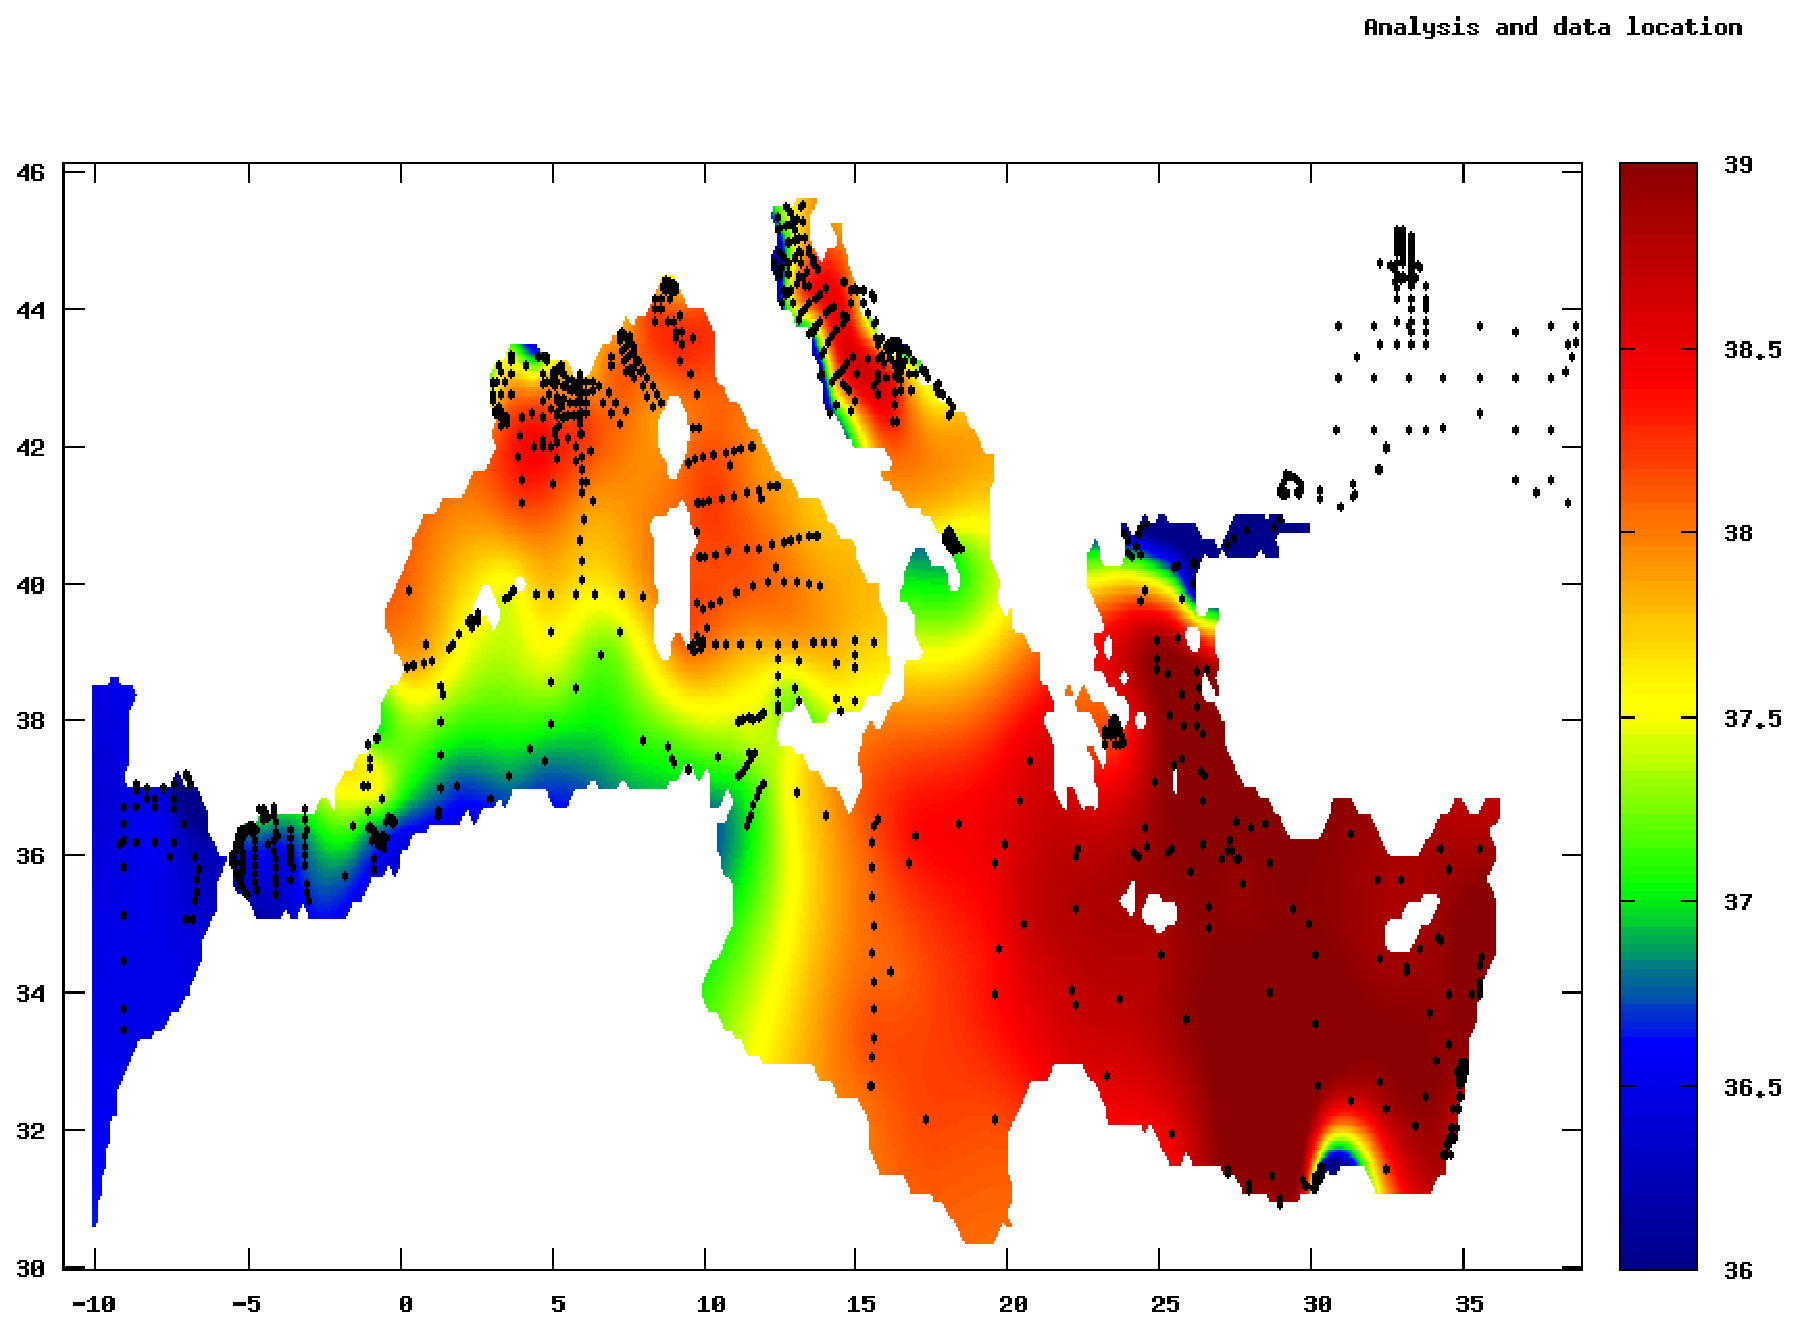
\includegraphics[width=0.9\textwidth]{diva_analysis_data}
}
\end{frame}

%---------------------------------------------------------------------

\begin{frame}{Estimation}
\begin{itemize}
\item
Observer 1: 14$^\circ$
\item
Observer 2: 16$^\circ$
\end{itemize}

\centerline{Your best guess ?}

\only<2->{\centerline{15$^\circ$}}
\only<3>{But what if observer 1 uses digital thermometer and observer 2 his finger ?}
\only<4>{But what if observer 1 uses digital thermometer and observer 2 his finger ?
\centerline{Best guess probably near 14$^\circ$.}}
\only<5>{But what if observer 1 uses digital thermometer and observer 2 his finger ?
\centerline{Best guess probably near 14$^\circ$.}
\begin{center}
\shabox{
Exploit knowledge of errors !}
\end{center}
}
\end{frame}

%---------------------------------------------------------------------

\begin{frame}{Optimal estimate}
\begin{equation}
T_1 = \true{T}+\epsilon_1, \quad \statmean{\epsilon_1} = 0, \quad T_2 = \true{T}+\epsilon_2, \quad \statmean{\epsilon_2} = 0
\end{equation}
statistical average, denoted by $\statmean{\quad}$ with unbiased estimates $\statmean{\epsilon_*}=0$

Linear estimate
\begin{equation}
{T}=w_1 \, T_1 ~+~ w_2 \, T_2 ~=~ (w_1+w_2) \true{T} ~+~ (w_1 \epsilon_1 + w_2 \epsilon_2)
\end{equation}
\begin{equation}
\statmean{{T}} = (w_1+w_2) \true{T},
\end{equation}
we obtain an unbiased estimate of the true state if we take $w_1+w_2=1$. This leaves one parameter free to chose: $w_2$
\begin{center}
\shabox{Exploit knowledge on errors to find optimal value of $w_2$}
\end{center}
\end{frame}

%---------------------------------------------------------------------

\begin{frame}{Choice of weighting ?}
\begin{equation}
\analyzed{T} = (1-w_2) T_1 + w_2 T_2  ~=~ T_1 + w_2 (T_2-T_1)
\end{equation}
while in reality there is an error
\begin{equation}
\analyzed{T} - \true{T} = (1-w_2) \epsilon_1 + w_2 \epsilon_2,
\end{equation}
This error is zero on average but its variance is not zero:
\begin{equation}
\statmean{(\analyzed{T}-\true{T})^2} = (1-w_2)^2 \statmean{\epsilon_1^2} + w_2^2 \statmean{\epsilon_2^2} + 2 (1-w_2) w_2 
\statmean{\epsilon_1 \epsilon_2}
\end{equation}
The actual errors $\epsilon_1$ and $\epsilon_2$ are not known, but the error variance $\statmean{\epsilon_1^2}$ are.
Often we can reasonably suppose that the errors
$\epsilon_1$ and $\epsilon_2$ are uncorrelated $\statmean{\epsilon_1 \epsilon_2}=0$. 
The error variance $\statmean{\epsilon^2}$ of the analysis is
\begin{equation}
\statmean{\epsilon^2}=(1-w_2)^2 \statmean{\epsilon_1^2} + w_2^2 \statmean{\epsilon_2^2}.
\label{eq:epsilonerror}
\end{equation}
So what ?
\end{frame}

%---------------------------------------------------------------------

\begin{frame}{Minimisation}
\begin{equation}
\statmean{\epsilon^2}=(1-w_2)^2 \statmean{\epsilon_1^2} + w_2^2 \statmean{\epsilon_2^2}.
\label{eq:epsilonerror}
\end{equation}
Naturally, the best estimate for $T$ is the one with the lowest expected error variance and we will use $w_2$, which minimizes
the right-hand side:
\begin{equation}
w_2 = \frac{\statmean{\epsilon_1^2}}{\statmean{\epsilon_1^2}+\statmean{\epsilon_2^2}}
\label{eq:weighterror}
\end{equation}
\begin{equation}
\analyzed{T}=   {\statmean{\epsilon_1^2} \statmean{\epsilon_2^2} \over \statmean{\epsilon_1^2} 
+ \statmean{\epsilon_2^2} }\left( {T_1 \over \statmean{\epsilon_1^2}} + {T_2 \over \statmean{\epsilon_2^2}}\right) .
 \label{eq:analyzedTb}
\end{equation}
\end{frame}

%---------------------------------------------------------------------

\begin{frame}{Best estimate}
With \eqref{eq:weighterror} we obtain the minimal error variance
\begin{equation}
\statmean{\epsilon^2}= {\statmean{\epsilon_1^2} \statmean{\epsilon_2^2} \over \statmean{\epsilon_1^2} 
+ \statmean{\epsilon_2^2} } = \left( 1 - {\statmean{\epsilon_1^2} \over \statmean{\epsilon_1^2} 
+ \statmean{\epsilon_2^2} } \right) \statmean{\epsilon_1^2},
\label{eq:optimalerror}
\end{equation}
while the estimate of the temperature itself reads
\begin{equation}
\analyzed{T}= T_1 ~+~ \left( {\statmean{\epsilon_1^2} \over \statmean{\epsilon_1^2} 
+ \statmean{\epsilon_2^2} } \right) \left( T_2-T_1\right).
 \label{eq:analyzedT}
\end{equation}
\begin{center}
\shabox{Error variance on the combination of $T_1$ and $T_2$ 
is smaller than both $\statmean{\epsilon_1^2}$ and $\statmean{\epsilon_2^2}$. }
\end{center}
\end{frame}

%---------------------------------------------------------------------

\begin{frame}[allowframebreaks]{Optimal Interpolation}
Same problem but data distributed in space and {\it a priori} information on background (with variance $\sigma^2$). 

Weighting of background (zero value when working with anomalies and $\sigma^2$ local variance and covariances between points) information and data points (observed values and observational error variance) 

\begin{itemize}
\item
"Model forecast": Background field.
\item
Need for  covariance of the background field between data points: each element $i,j$ of $\matr{B}$ provides the covariance between points in location $i$ and $j$. Covariance between a given point and all data points is stored in column vector $\matr{c}$ and the local variance at the analysis point is noted $\sigma^2$.
\item
Analysis $\phi$ of anomaly $\observation$ with respect to background leads to spatial analysis at any desired location of covariance between any two points is known.
\end{itemize}

\begin{equation}
\phi= {\matr{c}}^t \inv{\left( \matr{B} + \Rerr \right)} 
\observation
\label{eq:analyzedfield}
\end{equation}
with a local error variance of the analysis
\begin{equation}
\epsilon_a^2=\sigma^2 - {\matr{c}}^t \inv{\left( \matr{B} + \Rerr \right)} \matr{c}
\end{equation}
Note that inversion of matrix is needed (cost increases as the cube of number of data points).

\end{frame}

%---------------------------------------------------------------------

\begin{frame}{Background covariance}
Problem, how to specify background covariances (between all data points and between data points and the desired analysis location).
\begin{itemize}
\item $c_i$= {covariance between location of the analysis and data location of point i} = $C(x,x_i)$
\item $B_{ij}$={covariance between location of data point i and  location of point j}= $C(x_i,x_j)$
\end{itemize}
Approaches
\begin{itemize}
\item
Normally obtained via statistics on data. Seldom possible (noticable exception: satellite images).
\item
Standard OI: via functions $B_{ij}= f(r/L)$ where $r$ is the distance between points $i$ and $j$, but still function $f$ needs to be determined. $L$ is the so-called correlation length. Here statistics on all data couples as a function of distance.
Example: $f=\sigma^2 \exp(-r^2/L^2)$.
\item Via functionals (see Kernel of DIVA later)
\end{itemize}
\end{frame}

%---------------------------------------------------------------------

\begin{frame}{Signal to noise ratio}
\begin{equation}
\matr{B}= \sigma^2 \tilde{\matr{B}}
\end{equation}
\begin{equation}
\matr{R}= \epsilon^2 \tilde{\matr{R}}
\end{equation}
\begin{equation}
\matr{c}= \sigma^2 \tilde{\matr{c}}
\end{equation}
with non-dimensional correlation matrixes $\tilde{\matr{B}}$, $\tilde{\matr{R}}$, $\tilde{\matr{c}}$
\begin{equation}
\phi= {\tilde{\matr{c}}}^t \inv{\left( \tilde{\matr{B}} + {1 \over \lambda} \tilde{\Rerr} \right)} 
\observation
\label{eq:analyzedfield}
\end{equation}
with signal-to noise ratio
\begin{equation}
\lambda= {\sigma^2 \over \epsilon^2}
\end{equation}
Also the error field is only depending on the ratio.
\end{frame}

%---------------------------------------------------------------------
\begin{frame}[t]
\frametitle{DIVA: Data-Interpolating Variational Analysis}
\footnotesize

\begin{figure}[H]
\textcolor{blue}{$N_{d}$ data points $d_{i}$ $\bullet$}\quad $\rightarrow$ \quad{\textcolor{gray}{gridded field}}\\
\centering
\includegraphics[width=.4\textwidth,viewport=166   289   440   564]{gridding}
\end{figure}

\important{Formulation:} minimize cost function $J[\varphi]$


\begin{eqnarray*}
& &\min {J}[\varphi] = \sum_{i=1}^{N}\mu_i \left[d_{i}-\varphi(x_{i},y_{i})\right]^{2} \onslide<2->{\qquad\textcolor{gray}{\textrm{data--analysis misfit}}}\\
	  &+& \int_{{D}}\left(
{\nablab}{\nablab}\varphi : {\nablab}{\nablab}\varphi + { \alpha_{1}}
{\nablab}\varphi \cdot {\nablab}\varphi + \alpha_{0} \varphi^{2} \right) \ddiff {D} \onslide<2->{\qquad\textcolor{gray}{\textrm{field regularity}}}
\end{eqnarray*}

\end{frame}


%-----------------------------------------------------------------------------------------
\begin{frame}[t]
\frametitle{Analysis parameters are related to data}
\footnotesize

Non-dimensional version:

\begin{eqnarray}
L  = \textrm{length scale} &\rightarrow & \tilde{\nablab} = L \nablab\\
                     	   &\rightarrow & D = L^2 \tilde{D}
\end{eqnarray}

\onslide*<2->{
\begin{eqnarray*}
\tilde{J}[\varphi]&=&\sum_{i=1}^{N}\textcolor<5>{blue}{\mu_i L^2} [d_{i}-\varphi(x_{i},y_{i})]^{2}\\ 
&+&  \int_{\tilde{D}}\left(
 \tilde{\nablab}\tilde{\nablab}\varphi : \tilde{\nablab}\tilde{\nablab}\varphi + { \textcolor<4>{blue}{\alpha_{1}} L^2}
\tilde{\nablab}\varphi \cdot \tilde{\nablab}\varphi + \textcolor<3>{blue}{\alpha_{0}} L^4 \varphi^{2} \right) \ddiff \tilde{D}\nonumber
\end{eqnarray*}
}

\onslide*<3-5>{
\begin{itemize}
\item<3-> $\alpha_0$ \fleche $L$ for which data-analysis misfit $\simeq$ regularity term: \hspace*{\fill} $\alpha_0 L^4 = 1$

\item<4-> $\alpha_1$ \fleche influence of gradients: \hspace*{\fill}  $\alpha_1 L^2 = 2 \xi, \qquad \xi=1$

\item<5-> $ \mu_i L^2$ \fleche weight on data: \hspace*{\fill} 
$\displaystyle \mu_i L^2= 4 \pi \frac{\textrm{signal}}{\textrm{noise}_{i}}$
\end{itemize}
}

\onslide*<6>{
Coefficients $\alpha_0$, $\alpha_1$ and $\mu_i$ related to
\begin{enumerate}
\item Correlation length $L$
\item Signal-to-noise $\snr$
\item Observational noise standard deviation $\noise_i^2$
\end{enumerate}
}
\end{frame}

%---------------------------------------------------------------------------
\begin{frame}
\frametitle{Main analysis parameters}

\begin{columns}[totalwidth=\textwidth]
\column{.5\textwidth}
\important{Correlation length $L$:}

\begin{itemize}
\footnotesize
\item[]
\item Measure of the \textit{influence} of data points
\item Estimated by a least-square fit of the covariance function
\item[]
\end{itemize}

\important{Signal-to-noise ratio $\snr$:}

\begin{itemize}
\footnotesize
\item[]
\item Measure of the \textit{confidence} in data 
\item Estimated with Generalized Cross Validation techniques
\end{itemize}

\column{.5\textwidth}



\end{columns}


\end{frame}


%-------------------------------------------------------------------------------§
\begin{frame}
\footnotesize
\frametitle{Minimization with a finite-element method}

Field regularity \fleche plate bending problem \fleche finite-element solver

%Belgian specialties: finite-element mesh
\begin{figure}[H]
\centering
\includegraphics[width=.3\textwidth,viewport=165 273 429 567]{mesh_northsea}\includegraphics[width=.3\textwidth,viewport=133 272 448 568]{mesh_baltic}\includegraphics[width=.3\textwidth,viewport=138 272 443 568]{mesh_adriatic}
\end{figure}
\textbf{Advantages:}
\begin{itemize}
\item boundaries taken into account
\item numerical cost (almost independent on data number)
\item no \textit{a posteriori} masking (except if based on error level) 
\end{itemize}

\end{frame}

%----------------------------------------

\begin{frame}
\frametitle{Minimization with a finite-element method}
\footnotesize

%\begin{columns}[totalwidth=\textwidth]
%\column{.6\textwidth}

\onslide*<1>{

\begin{equation}
\textrm{Triangular FE only covers sea:}\qquad J[\varphi] = \sum_{e=1}^{N_{e}}J_{e}(\varphi_{e})
\label{eq:split}
\end{equation}

\begin{equation}
\textrm{In each element: } \varphi_{e}(\mathbf{r_e})=\mathbf{q_e}^{T}\mathbf{s}(\mathbf{r_e}) \quad \textrm{with} \left\{ \begin{array}{ll}
         \mathbf{s} & \rightarrow \mbox{shape functions}\\
         \mathbf{q} & \rightarrow  \mbox{\important{connectors}}\\
         \mathbf{r_e} & \rightarrow \mbox{position}
         \end{array} \right.
\label{eq:connectors}
\end{equation}

     
     
\eqref{eq:connectors} in \eqref{eq:split} + variational principle
\begin{equation}
J_{e}(\mathbf{q_e}) = \mathbf{q_e}^{T}\mathbf{K_e}\mathbf{q_e}-2\mathbf{q_e}^{T} \mathbf{g_{e}}+\sum_{i=1}^{N_{d_{e}}}\mu_{i}d_{i}
\label{eq:elements}
\end{equation}

\[ \quad\textrm{where }\left\{ \begin{array}{ll}
         \mathbf{K_e} & \rightarrow \mbox{local stiffness matrix}\\
         \mathbf{g} & \rightarrow  \mbox{vector depending on local data}
         \end{array} \right.
\]
}
      
      
\onslide*<2>{

\tikzstyle{na} = [baseline=-.5ex]
\begin{align}
\textrm{On the whole domain:}&&   J(\mathbf{q}) = \mathbf{q}^{T}\mathbf{K}\mathbf{q}-2\mathbf{q}^{T}\mathbf{g}+\sum_{i=1}^{N_{d}}\mu_{i}d_{i} &  \\
\textrm{Minimum:}&&  \mathbf{q}=\mathbf{K}^{-1}\mathbf{g}    & \\
&&    \tikz[baseline]{
            \node[fill=blue!30,anchor=base] (t1)
            {$\mathbf{q}$};
            } = 
        \tikz[baseline]{
            \node[fill=gray!30,anchor=base] (t2)
            {$\mathbf{K^{-1}}$};
        } 
        \tikz[baseline]{
            \node[fill=green!20,anchor=base] (t3)
        {$\mathbf{g}$};
        } & 
\end{align}

\begin{itemize}
\scriptsize
    \item Stiffness matrix
        \tikz[na]\node[coordinate] (n1) {};
    \item Connectors (new unknowns)
        \tikz[na]\node [coordinate] (n2) {};
    \item Charge vector
        \tikz[na]\node [coordinate] (n3) {};    
\end{itemize}
       
\begin{tikzpicture}[overlay]
\path[-] (n1) edge [out=0, in=-90] (t1);
\path[-] (n2) edge [out=0, in=-90] (t2);
\path[-] (n3) edge [out=0, in=-90] (t3);
\end{tikzpicture}

%$\mathbf{K}$ \fleche size proportional to $N_{\mathrm{dof}}$\\
%$\mathbf{K}^{-1}$ \fleche $N_{\mathrm{dof}}^{5/2}$ op. 

\begin{align*}
\textrm{Mapping of data on FEM} &\rightarrow & \textrm{transfer operator $\mathbf{T_{2}}$}&\rightarrow &\mathbf{g}=\mathbf{T_2}(\mathbf{r})\mathbf{d} \label{eq:T2}\\
\textrm{Solution at any location} &\rightarrow & \textrm{transfer operator $\mathbf{T_{1}}$}&\rightarrow &\boldsymbol{\varphi}(\mathbf{r})=\mathbf{T_1}(\mathbf{r})\mathbf{q}
%\label{eq:T1}
\end{align*}


\begin{align*}
\textrm{Results obtained at any location} \rightarrow  \boldsymbol{\varphi} = \mathbf{T_1}(\mathbf{r})\mathbf{K}^{-1}\mathbf{T_2}(\mathbf{r}) \mathbf{d} & &
%\label{eq:solution2}
\end{align*}

}
\end{frame}

%--------------------------------------------------------------------------------------------------------

\begin{frame}[t]
\frametitle{Diva Cocktail Recipe}

\begin{columns}[totalwidth=1.\textwidth]
\column{.65\textwidth}
\important{Ingredients:}
\onslide*<1>{
\begin{itemize}
\item 1 1/2 oz vodka
\item 1/2 oz passion-fruit juice
\item 1/2 oz lime juice
\item 1 tbsp cherry juice
\item fill with soda 
\end{itemize}
} 

\onslide*<2>{
\begin{itemize}
\item Smoothness \tikz[na] \coordinate (s-smooth);
\item Observation constraint \tikz[na] \coordinate (s-obs); 
\item Behaviour constraint \tikz[na] \coordinate (s-behaviour);
\end{itemize}
} 

\column{.35\textwidth}

\tikzstyle{background grid}=[draw, black!50,step=1cm]
\begin{tikzpicture}%[show background grid]
\node [inner sep=0pt,above right] 
{\includegraphics[width=.8\columnwidth]{cocktail}};
            % show origin
            %\fill (0,0) circle (2pt);
            % define destination coordinates
            \path (1.5,5.75) coordinate (smooth)
                  (0.4,1) coordinate (behaviour)
                  (0.4,3) coordinate (obs);
\end{tikzpicture}


\end{columns}
\onslide*<2>{
\begin{tikzpicture}[overlay]
        \path[-,black,thick] (s-smooth) edge (smooth);
        \path[-,black,thick] (s-obs) edge  (obs);
        \path[-,black,thick] (s-behaviour) edge  (behaviour);
\end{tikzpicture}
}
\end{frame}

%---------------------------------------------------------------------------------------------------
\begin{frame}[t]

\frametitle{Want to use \diva?}

\onslide*<1>{Playing\ldots}
\onslide*<2>{With your own data\ldots} 
\onslide*<3>{For serious work: \begin{description}
\item[2D version] (for production), open source, GPL 
\item[nD version] (for research), open source, GPL
\end{description}
}

%\begin{overlayarea}{\textwidth}{6.5cm}
\begin{figure}
\centering
\includegraphics<1>[width=.625\paperwidth]{diva_demo}
\includegraphics<2>[width=.8\paperwidth]{divaonweb}
\includegraphics<3>[width=.75\paperwidth]{divascreen}
\end{figure}
%\end{overlayarea}

\onslide*<1>{\footnotesize \url{http://data-assimilation.net/Tools/divand_demo/html/}}
\onslide*<2>{\footnotesize \url{http://gher-diva.phys.ulg.ac.be/web-vis/diva.html} or ODV or matlab wrapper}
\onslide*<3>{\footnotesize \url{http://modb.oce.ulg.ac.be/mediawiki/index.php/DIVA}}
\end{frame}

%-----------------------------------------------------------------------------------------------------------
\begin{frame}[t]
\frametitle{Running \diva in 2D: input files}

\begin{overlayarea}{\textwidth}{2cm}
\begin{enumerate}
\item<1-> \file{data.dat}: contains the observations \hfill \textcolor{gray}{x|y|value}
\item<2-> \file{coast.cont}: delimits land and sea \hfill \textcolor{gray}{(coastline or isobaths)}
\item<3-> \file{param.par}: analysis parameters \hfill \textcolor{gray}{$L$, $\lambda$, resolution, \ldots}
\end{enumerate}
\end{overlayarea}

\begin{figure}
\includegraphics<1>[height=.6\textheight]{datadat}
\includegraphics<2>[height=.6\textheight]{coastcont}
\includegraphics<3>[height=.6\textheight]{parampar}

\end{figure}
\end{frame}

%-----------------------------------------------------------------------------------------------------------
\begin{frame}[t]
\frametitle{Workflow in 2D}

\begin{overlayarea}{\textwidth}{.5cm}
\onslide*<1>{Select region of study}
\onslide*<2>{Extract \important{topography}, for example via {\tiny{\url{http://gher-diva.phys.ulg.ac.be/web-vis/diva.html}}}}
\onslide*<3>{Generate \important{contour}}
\onslide*<4>{Extract \important{data}}
\onslide*<5>{Evaluate analysis \important{parameters}}
\onslide*<6>{Create finite-element\important{ mesh}}
\onslide*<7>{Generate \important{analysis}}
\onslide*<8>{Generate \important{error} field}
\end{overlayarea}

\begin{figure}
\centering
\includegraphics<1>[width=.99\textwidth]{example2D_1_bs}
\includegraphics<2>[width=.89\textwidth]{example2D_2_bs}
\includegraphics<3>[width=.99\textwidth]{example2D_3_bs}
\includegraphics<4-5>[width=.99\textwidth]{example2D_4_bs}
\includegraphics<6>[width=.99\textwidth]{example2D_5_bs}
\includegraphics<7>[width=.99\textwidth]{example2D_6_bs}
\includegraphics<8>[width=.99\textwidth]{example2D_7_bs}
\end{figure}

\end{frame}
% 

\begin{frame}
\frametitle{When to use 2D version}
\begin{itemize}
\item occasional use
\item 2D fields like benthic properties
\item for implementation of special features by your own (eg multiplicative bias correction, special background field creation based on habitats 
\item ...
\end{itemize}
otherwise: use 3D or 4D version directly
\end{frame}

%-------------------------------------------------------------------------------------------------------------------------------------
\begin{frame}[c]
\frametitle{Next\ldots }
\huge
\diva in 4 dimensions

\end{frame}


\end{document}
